\chapter{Inclusión de la distancia temporal en el algoritmo de selección de
candidatos}
\label{ch:Cycle}

% Explicar el concepto de la distancia temporal con algún ejemplo.
\lettrine[lraise=-0.1, lines=2, loversize=0.2]{L}{a} idea de implementar una
distancia basada en ciclos surge de la observación realizada en los resultados de
la distancia de Levenshtein (ver subsección \ref{subsec:LevDicNoExhaust}). La
también llamada \textit{"distancia de ciclos"} se calcula a partir del primer 
ciclo en que la inyección se manifiesta a la salida, a partir de ahora 
\textit{"first cycle"}. La distancia de ciclos se calcula como la diferencia 
entre el \textit{first cycle} del target run y el \textit{first cycle} de cada 
entrada del diccionario, pudiendo ser positiva, negativa o cero si el fallo del 
target run se manifiesta antes, después o en el mismo ciclo que el de las 
entradas del diccionario.

% Decir las hipótesis realizadas para diagnosticar en base a la distancia de Cycle
    % Esta distancia no es nada sin la de levenshtein. Lev = 0 es que hemos i
    % terminado, cycle = 0 no implica Lev = 0
La hipótesis que realizamos basándonos en las observaciones y la cual aplicamos
para mejorar el diagnóstico sería la siguiente:
\begin{hypothesis}\label{hyp:cycle}
    "La distancia temporal, definida como la diferencia entre los primeros ciclos
    en que se manifiestan dos inyecciones, guarda relación directa con la
    diferencia entre los ciclos de inyección de dichas inyecciones".
\end{hypothesis}

Puntualizar que, mientras una distancia de Levenshtein nula significa que 
producen el mismo fallo a la salida y por tanto, bien son el mismo \gls{SEU} o 
bien colisionan; una distancia temporal nula no implica que nos encontremos ante
la misma inyección. Se cumple que:
\begin{center}
    $D_{Levenshtein} = 0 \Rightarrow D_{ciclo} = 0$
\end{center}

% Explicar que la base de datos de distancias se genera de forma similar
% dist = first_cycle[i] - target_first_cycle
Para generar la lista de distancias de ciclo entre el target run y el resto del
diccionario primero leemos la información de ambos archivos tal y como
explicábamos en la sección \ref{sec:LevenDist}. Después identificamos el primer
ciclo en que se manifiestan las inyecciones para cada entrada del diccionario.
Hacemos lo propio con el \gls{SEU} que estamos diagnosticando. La distancia de
ciclos se calcula como primer ciclo de la entrada menos primer ciclo del target
run. Se hace el cálculo para cada entrada del diccionario y se almacenan las
distancias temporales junto con las respectivas distancias de Levenshtein.

% Imagen ilustrativa cálculo de la distancia temporal
\begin{figure}[htbp]
    \centering
    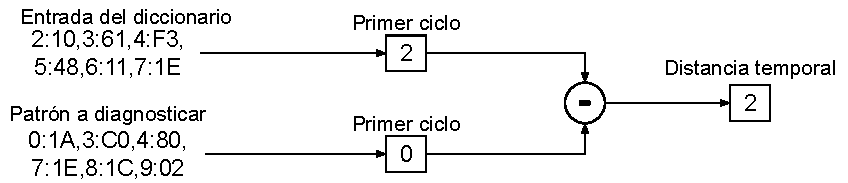
\includegraphics[width=0.95\linewidth]
    {Cycle/figuras/fig51.pdf}
    \caption{Cálculo de la distancia temporal}
    \label{fig:CycDist}
\end{figure}

% Decisiones tomada cuando el run es vacío y por qué
Al diagnosticar, suponemos que el target run presenta fallos a la salida, ya que
debe existir un error que detectar antes de saber que tenemos algo que
diagnosticar, por lo que siempre existirá primer ciclo para él. Esta afirmación no
es cierta para el resto de entradas del diccionario. Todas se corresponden con una
inyección, pero no todas producen errores a la salida. Esto se traduce en la
existencia de runs vacíos en el archivo \textit{"damages.csv"} y por tanto, en
entradas del diccionario a las cuales no se le puede asignar un \textit{first
cycle} de forma inmediata.

Cuando una inyección no se manifiesta a la salida puede deberse a tres razones
básicas:
% Solucion adoptada para esto
\begin{enumerate}
    \item El \gls{SEU} se produjo durante el reset, por lo que automáticamente se
        restaura el sistema.
    \item El \gls{SEU} no ha tenido tiempo suficiente para manifestarse a la
        salida.
    \item El \gls{SEU} esta localizado (FF, ciclo) en un sitio donde no produce
        fallos a la salida.
\end{enumerate}
Con la información que disponemos del propio diccionario, podemos identificar las
inyecciones que se han producido durante un reset del circuito y las que  se han
producido muy próxima al fin de su ejecución, no teniendo tiempo de manifestarse.

Aunque podríamos aproximar estos dos casos a primer ciclo cero y último
respectivamente, al final decidimos que lo mejor era descartar directamente los
runs vacíos como candidatos, ya que el target run siempre presenta fallos a la
salida y por tanto, en ningún caso puede corresponderse con una entrada del
diccionario vacía.

\section{Diagnóstico basado en la distancia temporal}
\label{sec:CycleCands}
% Explicar cómo se seleccionan los candidatos en base a las distancias calculadas
La selección de candidatos, en su versión final, la realizamos de la misma forma 
que para la distancie de Levenshtein con un ligero matiz. Las entradas del
diccionario se ordenan de menos a mayor según el valor absoluto de su distancia
temporal al target run. Una vez hecho esto, se seleccionan los \textit{"n"}
primeros.

El \gls{FF} de inyección de los candidatos seleccionados según la distancia
temporal no aporta información. Sin embargo, observamos cómo, en circuitos
simples, el ciclo donde se localiza el \gls{SEU} bajo diagnóstico coincide con 
la diferencia entre el ciclo de inyección del candidato y la distancia temporal 
que este presente hasta el target run. Para circuitos más grandes, con un mayor
número de biestables y que por tanto requieren ser ejecutados durante más ciclos
para que el diccionario presente las diferencias suficientes entre inyección e
inyección, observamos como este cálculo se aproxima bastante al valor del ciclo
real del target run. En la \textit{uart} por ejemplo, el margen de error oscila
en torno a los 1000 ciclos de los 37000 ciclos que componen cada ejecución.

Observamos además cómo el error cometido disminuye si lo hacemos con candidatos
que además dispongan de una distancia de Levenshtein relativamente baja.


\section{Fusión de las distancias temporal y de Levenshtein}
\label{sec:FusionLevenCycle}
% Puntos fuertes de cada algoritmo
El objetivo que perseguimos al fusionar las dos distancias es sacar partido de los
puntos fuertes de cada una de ellas.

Por un lado, la distancia de Levenshtein suele aproximarse más al registro e
incluso \gls{FF} correcto. Mientras que la distancia temporal resulta muy útil
para localizar temporalmente al \gls{SEU}.

% Explicar como se modifica el algotirmo para fusionar las dos distancias
El procedimiento que hemos seguido para diagnosticar conjuntamente con las dos
distancias consistía en calcular todas las distancias y agruparlas en una sola
lista, ordenar la lista de menor a mayor en función de la distancia de
Levenshtein y seleccionar los \textit{"n"} primeros.

% Cada candidato se muestra con las dos distancias auque sea seleccionado segun 
% una en concreto
Llegados a este punto, el algoritmo mostraba por pantalla, para cada candidato
seleccionado, su distancia de Levenshtein, su distancia de ciclo y la información
de su inyección. Además, dado que para nosotros esa información era conocida,
mostrábamos la localización correcta del \gls{SEU} a diagnosticar. Podíamos
comprobar cómo efectivamente, la inyección de los candidatos obtenido con la
distancia de Levenshtein podía ser corregida con la distancia temporal.

Más adelante, para la versión final de la técnica, contenida en el capítulo
\ref{ch:CampanasIterativas}, veremos cómo hemos integrado el cómputo del ciclo de
inyección completamente en el algoritmo.

\section{Resultados experimentales}
\label{sec:CycleResults}
Dado que la distancia temporal no está lo suficientemente basada en la salida 
como para realizar un diagnóstico completo únicamente a partir de ella, es difícil
mostrar unos resultados experimentales de este algoritmo aislado. Además, no fue
hasta más adelante, con la inclusión de dos aproximaciones más que aún faltan por
explicar, que empezamos a registrar resultados donde la distancia temporal 
intervenía.

Es por eso que a continuación vamos a ver sólo unos datos que se obtienen previos
a la fusión de las dos distancias.

\subsection{Diccionarios no exhaustivos}
\label{subsec:CycDicNoExhaust}
Dado que el diagnóstico con diccionarios exhaustivos se resuelve únicamente con la
distancia de Levenshtein, y esta investigación trata de desarrollar técnicas de
diagnóstico de \gls{SEU} con diccionarios incompletos, vamos a centrarnos
únicamente en los resultados que se obtienen con estos últimos.

% Tabla de resultados solo con leven. 5 cands, 5% o menos, reg
\begin{table}[htbp]
    \ttabbox
    {\caption{Resultados experimentales. Distancia de ciclos. Dic.
    incompletos ($\leq5\%$)}
    \label{tab:CycleRes}}
    {
        \begin{tabular}{c|c c}
            \hline
            \rule[-8pt]{0pt}{22pt}{\bfseries{Diseños}}&{\bfseries{Registro}}
            &{\bfseries{\gls{FF}}} \\
            \hline
            \rule{0pt}{14pt}adder\_acum & 100 & 37\\
            counter & 100 & 63\\
            dual\_counter & 98 & 67\\
            fifo & 98 & 0\\
            fir\_ri (37'78\%) & 21 & 4\\
            pcm & 67 & 52\\
            shiftreg & 100 & 52\\
            simple\_fsm & 100 & 88\\
            uart (0'87\%) & 92 & 74\\
            \hline
        \end{tabular}
    }
\end{table}

Los experimentos a partir de los cuales se han obtenido los datos de la tabla se
han realizado de la misma forma que la explicada en el capítulo anterior
(ver \ref{subsec:LevDicNoExhaust}), y los números representan también el número de
veces de las 100 simuladas que se encuentra el Registro/FF correcto entre los
candidatos.

Observamos cómo efectivamente se tiene menos capacidad de diagnóstico para 
\gls{FF} con la distancia de ciclo. Parece que además el porcentaje de acierto
ronda en torno al 50\%, lo cual encaja con la hipótesis de que la distancia
temporal no sirve más que para localizar el \gls{SEU} temporalmente, obteniendo
este nivel de acierto fruto del azar, aunque con excepciones.

Para el \textit{fifo} y el \textit{fir\_ri} el bajo nivel de acierto se explica
debido a una cantidad muy alta de colisiones. Además de los \textit{"n"} 
candidatos seleccionados hay muchos otros que son equidistantes a ellos y que no
se seleccionan, quedando atrás las inyecciones correctas a causa de las
colisiones.

Por el contrario, si que observamos circuitos donde se supera claramente la mitad
de aciertos. El caso de la máquina finita de estados se explica porque existen muy
pocos \gls{FF} donde seleccionar, por lo que es muy probable que uno de los
correctos se encuentre entre los candidatos. La \gls{UART} no tiene una
explicación tan sencilla. Puede deberse a la propia ejecución que está ejecutando.
Las zonas del circuito podrían estar activándose alternadamente por periodos, con
lo que al detectar los más próximos temporalmente, estaríamos seleccionando además
inyecciones a los mismos registros o incluso biestables.

\endinput
